\documentclass[10pt,a4paper]{amsart}
\usepackage[margin=19mm]{geometry}
\usepackage{amsmath,amssymb,mathtools}
\usepackage[scr=rsfs,cal=euler]{mathalfa}
\usepackage{xfrac}
\usepackage[unicode,hidelinks,bookmarks=false]{hyperref}
\newcommand{\ie}{i.e.\ }
\newcommand{\cf}{cf.\ }
\newcommand{\resp}{respectively\ }
\newcommand{\Subsection}{\subsection}
\providecommand{\nobreakdash}{\nobreak\hbox{-}}
\setlength{\emergencystretch}{2em}
\multlinegap0pt
\usepackage{tikz}
\usepackage{amssymb}
\usepackage{dsfont}
\usepackage{bm}
\newtheorem{thm}{Theorem}
\newtheorem{prop}{Proposition}
\newcommand{\bbE}{\mathbb{E}}
\newcommand{\bbN}{\mathbb{N}}
\newcommand{\bbP}{\mathbb{P}}
\newcommand{\bfX}{\mathbf{X}}
\newcommand{\calX}{\mathcal{X}}
\title{Genealogical processes of non-neutral population models under rapid mutation}
\author{Jere Koskela, Paul A. Jenkins, Adam M. Johansen, Dario Span\`o}
\date{Source: arXiv:2406.16465v3 (CC BY 4.0)}
\begin{document}
\maketitle

\noindent\emph{Source and licence.} Genealogical processes of non-neutral population models under rapid mutation. Version arXiv:2406.16465v3 (CC BY 4.0), distributed by arXiv under the Creative Commons Attribution 4.0 International licence, http://creativecommons.org/licenses/by/4.0/, as recorded in the arXiv licence metadata for this exact version and shown on the abstract page https://arxiv.org/abs/2406.16465v3. Full licence notice: \texttt{licenses/arxiv-2406.16465-CC-BY-4.0.txt}.\par\smallskip

\noindent\textit{Editorial scope.} Counted unit: the article's prop prop:stratified (source0.tex lines 588--603). The article's complete original proof of it is delivered with it (source0.tex lines 911--1097, one \texttt{proof} environment of 187 lines, which the article places away from the statement). No mathematics is written, repaired or re-derived: the statement and the proof are the article's own lines, in the article's own notation, and no retained line is substituted or re-flowed.  Retained uncounted as the source-local context the proof needs: lines 261--276; lines 263--269; lines 757--760; lines 763--766; lines 835--844; lines 863--865.  Nothing was omitted from any retained span, so the package carries no omission record.  No retained line contains a citation, so the wrapper carries no bibliography and no bibliography entry.  The retained lines contain the article's own diagram code, which the wrapper typesets with the standard tikz packages; no image file is delivered and the package declares no asset dependency.  Editorial formatting only, in addition: an AMS \texttt{amsart} preamble that restates the article's own declarations and macros used by the retained lines, namely the environments \texttt{thm}, \texttt{prop} on separate counters, together with the standard packages those lines need.  The retained environments print in this document as Theorem 1, Proposition 1 in order of appearance, whereas the article prints the same items with the numbering of its own full document.  The complete native source of the article as distributed in the arXiv e-print for this exact version is bundled unchanged as \texttt{sources/161267/source0.tex}.
\begin{thm}\label{thm:main_result}
Suppose that for any $n \in \bbN$, $j < k \in \bbN_0$, $t \in ( 0, \infty )$, any partition $\xi$ of $[n]$ and any $\eta$ such that $\xi \prec \eta$, and any $\ell \in [ N ]_d^{ | \xi | }$,
\begin{align}
\lim_{ N \to \infty } \bbE[ c_N( \xi, \ell, j; k ) | X_j ] &= 0, \label{kingman_assumption_1} \\
\lim_{ N \to \infty } \bbE[ c_N( \xi, \ell, j; \tau_N( \xi, \ell, j; t ) ) | X_j ] &= 0, \label{kingman_assumption_2} \\
\lim_{ N \to \infty } \bbE\Bigg[ \sum_{ k = j + 1 }^{ \tau_N( \xi, \ell, j; t ) } c_N( \xi, \ell, j; k )^2 \Big| X_j \Bigg] &= 0, \label{kingman_assumption_3} \\
\lim_{ N \to \infty } \frac{ \bbP^{ \bfX }( \bar{ G }_{ \tau_N( \xi, \ell, j; t ) }^{ N, n } = \eta | \bar{ G }_{ \tau_N( \xi, \ell, j; t ) - 1 }^{ N, n } = \xi, G_j^{ N, n } = ( \xi, \ell ) ) }{ c_N( \xi, \ell, j; \tau_N( \xi, \ell, j; t ) ) } &= 1, \label{kingman_assumption_4}\\
\lim_{N \to \infty} \bbP( \tau_N( \xi, \ell, j; t ) = \infty ) &= 0, \label{timescale_assumption}
\end{align}
hold $\bbP$-almost surely.
Then, for any fixed $n \in \bbN$,
\begin{equation*}
\lim_{ N \to \infty } ( \bar{ G }_{ \tau_N( t ) }^{ N, n } )_{ t \geq 0 } = ( \Pi_t^n )_{ t \geq 0 }
\end{equation*}
weakly in the Skorokhod $J_1$ topology on the space of right-continuous paths with left limits.
\end{thm}

\begin{align}
\lim_{ N \to \infty } \bbE[ c_N( \xi, \ell, j; k ) | X_j ] &= 0,  \\
\lim_{ N \to \infty } \bbE[ c_N( \xi, \ell, j; \tau_N( \xi, \ell, j; t ) ) | X_j ] &= 0,  \\
\lim_{ N \to \infty } \bbE\Bigg[ \sum_{ k = j + 1 }^{ \tau_N( \xi, \ell, j; t ) } c_N( \xi, \ell, j; k )^2 \Big| X_j \Bigg] &= 0,  \\
\lim_{ N \to \infty } \frac{ \bbP^{ \bfX }( \bar{ G }_{ \tau_N( \xi, \ell, j; t ) }^{ N, n } = \eta | \bar{ G }_{ \tau_N( \xi, \ell, j; t ) - 1 }^{ N, n } = \xi, G_j^{ N, n } = ( \xi, \ell ) ) }{ c_N( \xi, \ell, j; \tau_N( \xi, \ell, j; t ) ) } &= 1, \\
\lim_{N \to \infty} \bbP( \tau_N( \xi, \ell, j; t ) = \infty ) &= 0, 
\end{align}

\begin{align} 
&\bbP^{ \bfX }( | \bar{ G }_k^{ N, n } | < | \xi | - 1 | \bar{ G }_{ k - 1 }^{ N, n } = \xi, G_j^{ N, n } = ( \xi, \ell ) ) \notag \\
&\leq C_N^n \bbP^{ \bfX }( | \bar{ G }_k^{ N, n } | = | \xi | - 1 | \bar{ G }_{ k - 1 }^{ N, n } = \xi, G_j^{ N, n } = ( \xi, \ell ) ) ), \label{eq:large_mergers_vanish} 
\end{align}

\begin{align}
&\bbP^{ \bfX }( \bar{ G }_{ \tau_N( \xi, \ell, j; t ) }^{ N, n } = \eta | \bar{ G }_{ \tau_N( \xi, \ell, j; t ) - 1 }^{ N, n } = \xi, G_j^{ N, n } = ( \xi, \ell ) ) \notag \\
&\sim \binom{ | \xi | }{ 2 }^{ -1 } \bbP^{ \bfX }( | \bar{ G }_{ \tau_N( \xi, \ell, j; t ) }^{ N, n } | = | \xi | - 1  | \bar{ G }_{ \tau_N( \xi, \ell, j; t ) - 1 }^{ N, n } = \xi, G_j^{ N, n } = ( \xi, \ell ) ), \label{eq:binary_uniformity}
\end{align}

\begin{align}
&\bbP^{ \bfX }( \bar{ G }_{ \tau_N( \xi, \ell, j; t ) }^{ N, n } = \eta | \bar{ G }_{ \tau_N( \xi, \ell, j; t ) - 1 }^{ N, n } = \xi, G_j^{ N, n } = ( \xi, \ell ), \Xi ) \notag \\
&= \sum_{k = j + 1}^{\tau_N(\xi, \ell, j; t) - 1} \sum_{\ell' \in [N]_d^{|\xi|}} \bbP^{\bfX}(\bar{ G }_{ \tau_N( \xi, \ell, j; t ) }^{ N, n } = \eta | \bar{ G }_{ \tau_N( \xi, \ell, j; t ) - 1 }^{ N, n } = \xi, G_k^{N, n} = (\xi, \ell'), \Xi_k) \notag \\
&\mspace{166mu} \times \bbP^{\bfX}(\Xi_k, G_k^{ N, n } = ( \xi, \ell' ) | \bar{ G }_{ \tau_N( \xi, \ell, j; t ) - 1 }^{ N, n } = \xi, G_j^{ N, n } = ( \xi, \ell ), \Xi) \notag \\
&= \sum_{k = j + 1}^{\tau_N(\xi, \ell, j; t) - 1} \sum_{\ell' \in [N]_d^{|\xi|}} \bbP^{\bfX}(\bar{ G }_{ \tau_N( \xi, \ell, j; t ) }^{ N, n } = \eta | \bar{ G }_{ \tau_N( \xi, \ell, j; t ) - 1 }^{ N, n } = \xi, G_k^{N, n} = (\xi, \ell'), \Xi_k) \notag \\
&\mspace{166mu} \times \frac{\bbP^{\bfX}(\bar{ G }_{ \tau_N( \xi, \ell, j; t ) - 1 }^{ N, n } = \xi | G_k^{ N, n } = ( \xi, \ell' ), \Xi_k)}{\bbP^{\bfX}(\bar{ G }_{ \tau_N( \xi, \ell, j; t ) - 1 }^{ N, n } = \xi | G_j^{ N, n } = ( \xi, \ell ), \Xi)} \notag \\
&\mspace{166mu} \times \bbP^{\bfX}(\Xi_k, G_k^{ N, n } = ( \xi, \ell' ) | G_j^{ N, n } = ( \xi, \ell ), \Xi) \notag \\
&= \sum_{k = j + 1}^{\tau_N(\xi, \ell, j; t) - 1} \sum_{\ell' \in [N]_d^{|\xi|}} \frac{\bbP^{\bfX}(\bar{ G }_{ \tau_N( \xi, \ell, j; t ) }^{ N, n } = \eta, \bar{ G }_{ \tau_N( \xi, \ell, j; t ) - 1 }^{ N, n } = \xi | G_k^{N, n} = (\xi, \ell'), \Xi_k)}{\bbP^{\bfX}(\bar{ G }_{ \tau_N( \xi, \ell, j; t ) - 1 }^{ N, n } = \xi | G_j^{ N, n } = ( \xi, \ell ), \Xi)}\notag \\
&\mspace{166mu} \times \frac{(1 - \gamma^{-2 |\xi|})^{k - j - 1} \gamma^{-2|\xi|}}{N^{|\xi|} (1 - (1 - \gamma^{-2 |\xi|})^{\tau_N(\xi, \ell, j;t) - j - 1})}, \label{eq:label_mixing}
\end{align}

\begin{equation}\label{binomial_sum}
\sum_{j = 2}^n \binom{j}{2} = \frac{(n + 1) n (n - 1)}{6}.
\end{equation}

\begin{prop}\label{prop:stratified}
Suppose there exists $\gamma \geq 1$, a function $f : \calX \to ( 0, \infty )$, and a sequence $\varepsilon_N > 0$ such that
\begin{align}
\frac{ f( y ) }{ \sqrt{ \gamma } } &\leq M_k( x, y ) \leq \sqrt{ \gamma } f( y ), \label{eq:m_mixing} \\
\frac{ 1 }{ \sqrt{ \gamma } } &\leq g_k( x ) \leq \sqrt{ \gamma }, \label{eq:uniform_weight_bound} \\
\lim_{ N \to \infty } &\bbP( \bfX : \max_{ i \in [ N ] }\{ \bar{ g }_k^{ ( i ) } - \bar{g}_k^{ ( i - 1 ) } \} > 1 / N + \varepsilon_N ) = 1, \label{eq:environment}
\end{align}
for each $x \in \calX$ and $k \geq 1$.
Then stratified resampling with uniform shuffling satisfies the conditions of Theorem \ref{thm:main_result}.
Moreover, the timescale $\tau_N(t)$ satisfies
\begin{align}
\Big\lfloor (1 + o(1)) \frac{N t}{\gamma^4} \Big\rfloor &\leq \tau_N(t) \text{ a.s.}, \label{stratified_timescale_lb}\\
\lim_{N \to \infty} \bbP\Bigg( \tau_N(t) \leq \frac{(n + 1) n (n - 1)}{6} \Big\lceil \frac{\gamma^2 N t}{\varepsilon_N} \Big\rceil \Bigg) &\to 1, \label{stratified_timescale_ub}
\end{align}
for any fixed initial sample size $n \leq N$.
\end{prop}

\begin{proof}[Proof of Proposition \ref{prop:stratified}]
Under stratified resampling, the conditional probability given $\bfX$ that particle $\ell \in [N]$ in generation $k - 1$ has parent $m \in [N]$ in generation $k$ is
\begin{equation*}
\frac{ | [ \frac{ \ell - 1 }{ N }, \frac{ \ell }{ N } ) \cap [ \bar{ g }_k^{ ( m - 1 ) }, \bar{ g }_k^{ ( m ) } ) | M_k( X_k( m ), X_{ k - 1 }( \ell ) ) }{ \sum_{ h = 1 }^N | [ \frac{ \ell - 1 }{ N }, \frac{ \ell }{ N } ) \cap [ \bar{ g }_k^{ ( h - 1 ) }, \bar{ g }_k^{ ( h ) } ) | M_k( X_k( h ), X_{ k - 1 }( \ell ) ) }.
\end{equation*}
Thus, the conditional probability of at least one merger in generation $k$ among $| \xi |$ lineages can be bounded above by conditioning on the uniformly sampled indices $( h_1, \ldots, h_{ | \xi | } )$ to which they are shuffled, and multiplying by the probability that at least two of those indices obtain the same parent in the stratified resampling scheme:
\begin{align*}
&\bbP^{ \bfX }( | \bar{ G }_k^{ N, n } | < | \xi | | \bar{ G }_{ k - 1 }^{ N, n } = \xi, G_j^{ N, n } = ( \xi, \ell_0 ) ) \\
&\leq \sum_{ \ell_1 \in [ N ]_d^{ | \xi | } } \bbP^{ \bfX }( G_{ k - 1 }^{ N, n } = ( \xi, \ell_1 ) | \bar{ G }_{ k - 1 }^{ N, n } = \xi, G_j^{ N, n } = ( \xi, \ell_0 ) ) \sum_{ ( h_1, \ldots, h_{ | \xi | } ) \in [ N ]_d^{ | \xi | } }  \frac{ 1 }{ ( N )_{ | \xi | } } \\
&\phantom{=} \times \sum_{ ( v_1, v_2 ) \in [ | \xi | ]_{ d, u }^2 } \sum_{ m = 1 }^N \prod_{ i \in \{ 1, 2 \} } \frac{ | [ \frac{ h_{ v_i } - 1 }{ N }, \frac{ h_{ v_i } }{ N } ) \cap [ \bar{ g }_k^{ ( m - 1 ) }, \bar{ g }_k^{ ( m ) } ) | M_k( X_k( m ), X_{ k - 1 }( \ell_1^{ v_i } ) ) }{ \sum_{ r = 1 }^N | [ \frac{ h_{ v_i } - 1 }{ N }, \frac{ h_{ v_i } }{ N } ) \cap [ \bar{ g }_k^{ ( r - 1 ) }, \bar{ g }_k^{ ( r ) } ) | M_k( X_k( r ), X_{ k - 1 }( \ell_1^{ v_i } ) ) } \\
&= \sum_{ \ell_1 \in [ N ]_d^{ | \xi | } } \bbP^{ \bfX }( G_{ k - 1 }^{ N, n } = ( \xi, \ell_1 ) | \bar{ G }_{ k - 1 }^{ N, n } = \xi, G_0^{ N, n } = ( \xi, \ell_0 ) ) \sum_{ ( v_1, v_2 ) \in [ | \xi | ]_{ d, u }^2 } \sum_{ ( h_{ v_1 }, h_{ v_2 } ) \in [ N ]_d^2 } \\
&\phantom{=} \frac{ 1 }{ ( N )_2 } \sum_{ m = 1 }^N \prod_{ i \in \{ 1, 2 \} } \frac{ | [ \frac{ h_{ v_i } - 1 }{ N }, \frac{ h_{ v_i } }{ N } ) \cap [ \bar{ g }_k^{ ( m - 1 ) }, \bar{ g }_k^{ ( m ) } ) | M_k( X_k( m ), X_{ k - 1 }( \ell_1^{ v_i } ) ) }{ \sum_{ r = 1 }^N | [ \frac{ h_{ v_i } - 1 }{ N }, \frac{ h_{ v_i } }{ N } ) \cap [ \bar{ g }_k^{ ( r - 1 ) }, \bar{ g }_k^{ ( r ) } ) | M_k( X_k( r ), X_{ k - 1 }( \ell_1^{ v_i } ) ) },
\end{align*}
where the inequality arises because the right-hand side overcounts some mergers.
Applying \eqref{eq:m_mixing} to the last line, we obtain
\begin{align}
&\bbP^{ \bfX }( | \bar{ G }_k^{ N, n } | < | \xi | | \bar{ G }_{ k - 1 }^{ N, n } = \xi, G_j^{ N, n } = ( \xi, \ell_0 ) ) \notag \\
&\leq \frac{ \gamma^2 }{ ( N )_2 } \sum_{ \ell_1 \in [ N ]_d^{ | \xi | } } \bbP^{ \bfX }( G_{ k - 1 }^{ N, n } = ( \xi, \ell_1 ) | \bar{ G }_{ k - 1 }^{ N, n } = \xi, G_j^{ N, n } = ( \xi, \ell_0 ) ) \notag \\
&\phantom{= \sum_{ \ell_1 \in [ N ]_d^{ | \xi | } } } \times \sum_{ ( v_1, v_2 ) \in [ | \xi | ]_{ d, u }^2 } \sum_{ ( h_{ v_1 }, h_{ v_2 } ) \in [ N ]_d^2 } \sum_{ m = 1 }^N \prod_{ i \in \{ 1, 2 \} } \frac{ | [ \frac{ h_{ v_i } - 1 }{ N }, \frac{ h_{ v_i } }{ N } ) \cap [ \bar{ g }_k^{ ( m - 1 ) }, \bar{ g }_k^{ ( m ) } ) | }{ \sum_{ r = 1 }^N | [ \frac{ h_{ v_i } - 1 }{ N }, \frac{ h_{ v_i } }{ N } ) \cap [ \bar{ g }_k^{ ( r - 1 ) }, \bar{ g }_k^{ ( r ) } ) | } \notag \\
&\leq \frac{ \gamma^2 }{ ( N )_2 } \binom{ | \xi | }{ 2 } \sum_{ \ell_1 \in [ N ]_d^{ | \xi | } } \bbP^{ \bfX }( G_{ k - 1 }^{ N, n } = ( \xi, \ell_1 ) | \bar{ G }_{ k - 1 }^{ N, n } = \xi, G_j^{ N, n } = ( \xi, \ell_0 ) ) \notag \\
&\phantom{\leq \frac{ \gamma^4 }{ ( N )_2 } \binom{ | \xi | }{ 2 } \sum_{ \ell_1 \in [ N ]_d^{ | \xi | } } } \times \sum_{ ( h_1, h_2 ) \in [ N ]_d^2 } \sum_{ m = 1 }^N \prod_{ i \in \{ 1, 2 \} } \frac{ | [ \frac{ h_i - 1 }{ N }, \frac{ h_i }{ N } ) \cap [ \bar{ g }_k^{ ( m - 1 ) }, \bar{ g }_k^{ ( m ) } ) | }{ \sum_{ r = 1 }^N | [ \frac{ h_i - 1 }{ N }, \frac{ h_i }{ N } ) \cap [ \bar{ g }_k^{ ( r - 1 ) }, \bar{ g }_k^{ ( r ) } ) | }. \label{sum_rearrangement}
\end{align}
For fixed $h_i$, the sum in the denominator on the last line simplifies to
\begin{equation}\label{eq:stratified_denominator}
\sum_{ r = 1 }^N  \Big| \Big[ \frac{ h_i - 1 }{ N }, \frac{ h_i }{ N } \Big) \cap [ \bar{ g }_k^{ ( r - 1 ) }, \bar{ g }_k^{ ( r ) } ) \Big| = \Big| \Big[ \frac{ h_i - 1 }{ N }, \frac{ h_i }{ N } \Big) \Big| = \frac{ 1 }{ N },
\end{equation}
so that
\begin{align}
&\bbP^{ \bfX }( | \bar{ G }_k^{ N, n } | < | \xi | | \bar{ G }_{ k - 1 }^{ N, n } = \xi, G_j^{ N, n } = ( \xi, \ell_0 ) ) \notag \\
&\leq \sum_{ \ell_1 \in [ N ]_d^{ | \xi | } } \bbP^{ \bfX }( G_{ k - 1 }^{ N, n } = ( \xi, \ell_1 ) | \bar{ G }_{ k - 1 }^{ N, n } = \xi, G_j^{ N, n } = ( \xi, \ell_0 ) ) \notag \\
&\phantom{ \leq \sum_{ \ell_1 \in [ N ]_d^{ | \xi | } } } \times \frac{ N \gamma^2 }{ N - 1 } \binom{ | \xi | }{ 2 } \sum_{ ( h_1, h_2 ) \in [ N ]_d^2 } \sum_{ m = 1 }^N \prod_{ i \in \{ 1, 2 \} } \Big| \Big[ \frac{ h_i - 1 }{ N }, \frac{ h_i }{ N } \Big) \cap [ \bar{ g }_k^{ ( m - 1 ) }, \bar{ g }_k^{ ( m ) } ) \Big|. \label{eq:stratified_ub_1}
\end{align}
For a fixed $m$, we have the bound
\begin{align}
&\sum_{ ( h_1, h_2 ) \in [ N ]_d^2 } \prod_{ i \in \{ 1, 2 \} } \Big| \Big[ \frac{ h_i - 1 }{ N }, \frac{ h_i }{ N } \Big) \cap [ \bar{ g }_k^{ ( m - 1 ) }, \bar{ g }_k^{ ( m ) } ) \Big| \notag \\
&\leq \Bigg( \sum_{ h = 1 }^N \Big| \Big[ \frac{ h - 1 }{ N }, \frac{ h }{ N } \Big) \cap [ \bar{ g }_k^{ ( m - 1 ) }, \bar{ g }_k^{ ( m ) } ) \Big| \Bigg)^2 = | [ \bar{ g }_k^{ ( m - 1 ) }, \bar{ g }_k^{ ( m ) } ) |^2 \leq \frac{ \gamma^2 }{ N^2 }, \label{eq:stratified_numerator}
\end{align}
where the final inequality follows from \eqref{eq:uniform_weight_bound}.
Substituting back into \eqref{eq:stratified_ub_1},
\begin{align}
&\bbP^{ \bfX }( | \bar{ G }_k^{ N, n } | < | \xi | | \bar{ G }_{ k - 1 }^{ N, n } = \xi, G_j^{ N, n } = ( \xi, \ell_0 ) ) \notag \\
&\leq \sum_{ \ell_1 \in [ N ]_d^{ | \xi | } } \bbP^{ \bfX }( G_{ k - 1 }^{ N, n } = ( \xi, \ell_1 ) | \bar{ G }_{ k - 1 }^{ N, n } = \xi, G_j^{ N, n } = ( \xi, \ell_0 ) ) \frac{ N \gamma^2 }{ N - 1 } \frac{ \gamma^2 }{ N } \binom{ | \xi | }{ 2 } \notag \\
&= \frac{ \gamma^4 ( 1 + o( 1 ) ) }{ N } \binom{ | \xi | }{ 2 }, \label{eq:stratified_merger_ub}
\end{align}
where the sum over $[ N ]_d^{ | \xi | }$ evaluates to one because it adds up a conditional probability mass function over its support.
Similarly to the multinomial case, this upper bound on the binary merger probability means that \eqref{kingman_assumption_1}, \eqref{kingman_assumption_2}, and \eqref{kingman_assumption_3} hold.

As with multinomial resampling, \eqref{eq:large_mergers_vanish} and \eqref{eq:binary_uniformity} are a sufficient condition for \eqref{kingman_assumption_4}.
To show that \eqref{eq:large_mergers_vanish} holds, we write the probability of the number of blocks decreasing by more than one as
\begin{align*}
&\bbP^{ \bfX }( | \bar{ G }_k^{ N, n } | < | \xi | - 1 | \bar{ G }_{ k - 1 }^{ N, n } = \xi, G_j^{ N, n } = ( \xi, \ell ) ) \\
&= \sum_{ \ell_1 \in [ N ]_d^{ | \xi | } } \bbP^{ \bfX }( | \bar{ G }_k^{ N, n } | < | \xi | - 1 | G_{ k - 1 }^{ N, n } = ( \xi, \ell_1 ) )  \bbP^{ \bfX }( G_{ k - 1 }^{ N, n } = ( \xi, \ell_1 ) | \bar{ G }_{ k - 1 }^{ N, n } = \xi, G_j^{ N, n } = ( \xi, \ell_0 ) ) \\
&\leq \sum_{ \ell_1 \in [ N ]_d^{ | \xi | } } \bbP^{ \bfX }( G_{ k - 1 }^{ N, n } = ( \xi, \ell_1 ) | \bar{ G }_{ k - 1 }^{ N, n } = \xi, G_j^{ N, n } = ( \xi, \ell_0 ) )  \sum_{ ( h_1, \ldots, h_{ | \xi | } ) \in [ N ]_d^{ | \xi | } }  \frac{ 1 }{ ( N )_{ | \xi | } } \\
&\phantom{\leq} \times \sum_{ ( v_1, v_2 ) \in [ | \xi | ]_{ d, u }^2 } \sum_{ m = 1 }^N \Bigg( \prod_{ i = 1 }^2 \frac{ | [ \frac{ h_{ v_i } - 1 }{ N }, \frac{ h_{ v_i } }{ N } ) \cap [ \bar{ g }_k^{ ( m - 1 ) }, \bar{ g }_k^{ ( m ) } ) | M_k( X_k( m ), X_{ k - 1 }( \ell_1^{ v_i } ) ) }{ \sum_{ r = 1 }^N | [ \frac{ h_{ v_i } - 1 }{ N }, \frac{ h_{ v_i } }{ N } ) \cap [ \bar{ g }_k^{ ( r - 1 ) }, \bar{ g }_k^{ ( r ) } ) | M_k( X_k( r ), X_{ k - 1 }( \ell_1^{ v_i } ) ) } \Bigg) \\
&\phantom{\leq} \times \Bigg[ \frac{ 1 }{ 3 } \sum_{ v_3 \neq v_1, v_2 } \frac{ | [ \frac{ h_{ v_3 } - 1 }{ N }, \frac{ h_{ v_3 } }{ N } ) \cap [ \bar{ g }_k^{ ( m - 1 ) }, \bar{ g }_k^{ ( m ) } ) | M_k( X_k( m ), X_{ k - 1 }( \ell_1^{ v_3 } ) ) }{ \sum_{ r = 1 }^N | [ \frac{ h_{ v_3 } - 1 }{ N }, \frac{ h_{ v_3 } }{ N } ) \cap [ \bar{ g }_k^{ ( r - 1 ) }, \bar{ g }_k^{ ( r ) } ) | M_k( X_k( r ), X_{ k - 1 }( \ell_1^{ v_3 } ) ) } + \frac{ 1 }{ 2 } \\
&\phantom{\times \Bigg[} \times \sum_{ \substack{ ( v_3, v_4 ) \in [ | \xi | ]_{ d, u }^2 \\ \text{both } \neq v_1, v_2 } } \sum_{ m' \neq m } \prod_{ i = 3 }^4 \frac{ | [ \frac{ h_{ v_i } - 1 }{ N }, \frac{ h_{ v_i } }{ N } ) \cap [ \bar{ g }_k^{ ( m' - 1 ) }, \bar{ g }_k^{ ( m' ) } ) | M_k( X_k( m' ), X_{ k - 1 }( \ell_1^{ v_i } ) ) }{ \sum_{ r = 1 }^N | [ \frac{ h_{ v_i } - 1 }{ N }, \frac{ h_{ v_i } }{ N } ) \cap [ \bar{ g }_k^{ ( r - 1 ) }, \bar{ g }_k^{ ( r ) } ) | M_k( X_k( r ), X_{ k - 1 }( \ell_1^{ v_i } ) ) } \Bigg],
\end{align*}
where the right-hand side is an upper bound on the probabilities of a merger of three lineages, or two simultaneous mergers of a pair of lineages each.
All larger mergers must contain at least one of these events.
Applying \eqref{eq:m_mixing} and \eqref{eq:stratified_denominator} to the terms in square brackets and simplifying the sum over $( h_1, \ldots, h_{ | \xi | } )$ similarly to \eqref{sum_rearrangement}, 
\begin{align}
&\bbP^{ \bfX }( | \bar{ G }_k^{ N, n } | < | \xi | - 1 | \bar{ G }_{ k - 1 }^{ N, n } = \xi, G_j^{ N, n } = ( \xi, \ell ) ) \notag \\
&\leq \sum_{ \ell_1 \in [ N ]_d^{ | \xi | } } \bbP^{ \bfX }( G_{ k - 1 }^{ N, n } = ( \xi, \ell_1 ) | \bar{ G }_{ k - 1 }^{ N, n } = \xi, G_j^{ N, n } = ( \xi, \ell_0 ) ) \sum_{ ( v_1, v_2 ) \in [ | \xi | ]_{ d, u }^2 } \frac{ 1 }{ ( N )_2 } \notag \\
&\phantom{\leq} \times \sum_{ ( h_1, h_2 ) \in [ N ]_d^2 } \sum_{ m = 1 }^N \Bigg( \prod_{ i = 1 }^2 \frac{ | [ \frac{ h_i - 1 }{ N }, \frac{ h_i }{ N } ) \cap [ \bar{ g }_k^{ ( m - 1 ) }, \bar{ g }_k^{ ( m ) } ) | M_k( X_k( m ), X_{ k - 1 }( \ell_1^{ v_i } ) ) }{ \sum_{ r = 1 }^N | [ \frac{ h_i - 1 }{ N }, \frac{ h_i }{ N } ) \cap [ \bar{ g }_k^{ ( r - 1 ) }, \bar{ g }_k^{ ( r ) } ) | M_k( X_k( r ), X_{ k - 1 }( \ell_1^{ v_i } ) ) } \Bigg) \notag \\
&\phantom{\leq \times } \times \Bigg[ \frac{ N \gamma  ( | \xi | - 2 ) }{ 3 ( N - 2 ) } \sum_{ h_3 \neq h_1, h_2 } \Big| \Big[ \frac{ h_3 - 1 }{ N }, \frac{ h_3 }{ N } \Big) \cap [ \bar{ g }_k^{ ( m - 1 ) }, \bar{ g }_k^{ ( m ) } ) \Big| \notag \\
&\phantom{\leq \times \times \Bigg[} + \frac{ ( N \gamma )^2 }{ 2 ( N - 2 )_2 } \binom{ | \xi | - 2 }{ 2 }  \sum_{ \substack{ ( h_3, h_4 ) \in [ N ]_d^2 \\ \text{both } \neq h_1, h_2 } } \sum_{ m' \neq m } \prod_{ i = 3 }^4 \Big| \Big[ \frac{ h_i - 1 }{ N }, \frac{ h_i }{ N } \Big) \cap [ \bar{ g }_k^{ ( m' - 1 ) }, \bar{ g }_k^{ ( m' ) } ) \Big| \Bigg]. \label{eq:stratified_multiple_merger_bound}
\end{align}
Similarly to \eqref{eq:stratified_numerator}, we have the bounds
\begin{align*}
\sum_{ h_3 \neq h_1, h_2 } \Big| \Big[ \frac{ h_3 - 1 }{ N }, \frac{ h_3 }{ N } \Big) \cap [ \bar{ g }_k^{ ( m - 1 ) }, \bar{ g }_k^{ ( m ) } ) \Big| &\leq\frac{ \gamma }{ N }, \\
\sum_{ \substack{ ( h_3, h_4 ) \in [ N ]_d^2 \\ \text{both } \neq h_1, h_2 } } \sum_{ m' \neq m } \prod_{ i = 3 }^4 \Big| \Big[ \frac{ h_i - 1 }{ N }, \frac{ h_i }{ N } \Big) \cap [ \bar{ g }_k^{ ( m' - 1 ) }, \bar{ g }_k^{ ( m' ) } ) \Big| &\leq \frac{ \gamma^2 }{ N }.
\end{align*}
Substituting these into \eqref{eq:stratified_multiple_merger_bound} yields
\begin{align*}
&\bbP^{ \bfX }( | \bar{ G }_k^{ N, n } | < | \xi | - 1 | \bar{ G }_{ k - 1 }^{ N, n } = \xi, G_j^{ N, n } = ( \xi, \ell ) ) \\
&\leq \sum_{ \ell_1 \in [ N ]_d^{ | \xi | } } \bbP^{ \bfX }( G_{ k - 1 }^{ N, n } = ( \xi, \ell_1 ) | \bar{ G }_{ k - 1 }^{ N, n } = \xi, G_j^{ N, n } = ( \xi, \ell_0 ) ) \frac{ \gamma^2 }{ ( N )_3 } \Bigg[ \frac{ | \xi | - 2 }{ 3 } + \frac{ N \gamma^2 }{ 2 ( N - 3 ) } \binom{ | \xi | - 2 }{ 2 } \Bigg]\\
&\phantom{\leq} \times  \sum_{ ( v_1, v_2 ) \in [ | \xi | ]_{ d, u }^2 } \sum_{ ( h_1, h_2 ) \in [ N ]_d^2 } \sum_{ m = 1 }^N  \prod_{ i = 1 }^2 \frac{ | [ \frac{ h_i - 1 }{ N }, \frac{ h_i }{ N } ) \cap [ \bar{ g }_k^{ ( m - 1 ) }, \bar{ g }_k^{ ( m ) } ) | M_k( X_k( m ), X_{ k - 1 }( \ell_1^{ v_i } ) ) }{ \sum_{ r = 1 }^N | [ \frac{ h_i - 1 }{ N }, \frac{ h_i }{ N } ) \cap [ \bar{ g }_k^{ ( r - 1 ) }, \bar{ g }_k^{ ( r ) } ) | M_k( X_k( r ), X_{ k - 1 }( \ell_1^{ v_i } ) ) }.
\end{align*}
To obtain the required bound, the right-hand side must be bounded above by the product of $\bbP^{ \bfX }( | \bar{ G }_k^{ N, n } | < | \xi | | \bar{ G }_{ k - 1 }^{ N, n } = \xi, G_j^{ N, n } = ( \xi, \ell ) )$ and a factor tending to zero as $N \to \infty$.
Currently, the sum over $( v_1, v_2 ) \in [ | \xi | ]_{ d, u }^2$ overcounts mergers involving more than two lineages.
By \eqref{eq:m_mixing}, 
\begin{align*}
&\frac{ | [ \frac{ h_i - 1 }{ N }, \frac{ h_i }{ N } ) \cap [ \bar{ g }_k^{ ( m - 1 ) }, \bar{ g }_k^{ ( m ) } ) | M_k( X_k( m ), X_{ k - 1 }( \ell_1^{ v_i } ) ) }{ \sum_{ r = 1 }^N | [ \frac{ h_i - 1 }{ N }, \frac{ h_i }{ N } ) \cap [ \bar{ g }_k^{ ( r - 1 ) }, \bar{ g }_k^{ ( r ) } ) | M_k( X_k( r ), X_{ k - 1 }( \ell_1^{ v_i } ) ) } \\
&\leq \gamma^2 \frac{ | [ \frac{ h_i - 1 }{ N }, \frac{ h_i }{ N } ) \cap [ \bar{ g }_k^{ ( m - 1 ) }, \bar{ g }_k^{ ( m ) } ) | M_k( X_k( m ), X_{ k - 1 }( \ell_1^i ) ) }{ \sum_{ r = 1 }^N | [ \frac{ h_i - 1 }{ N }, \frac{ h_i }{ N } ) \cap [ \bar{ g }_k^{ ( r - 1 ) }, \bar{ g }_k^{ ( r ) } ) | M_k( X_k( r ), X_{ k - 1 }( \ell_1^i ) ) }
\end{align*}
for $v_i, i \in [ | \xi | ]$, so that
\begin{align*}
&\bbP^{ \bfX }( | \bar{ G }_k^{ N, n } | < | \xi | - 1 | \bar{ G }_{ k - 1 }^{ N, n } = \xi, G_j^{ N, n } = ( \xi, \ell ) ) \\
&\leq \sum_{ \ell_1 \in [ N ]_d^{ | \xi | } } \bbP^{ \bfX }( G_{ k - 1 }^{ N, n } = ( \xi, \ell_1 ) | \bar{ G }_{ k - 1 }^{ N, n } = \xi, G_j^{ N, n } = ( \xi, \ell_0 ) )  \frac{ \gamma^6 ( | \xi | - 2 ) }{ N - 2 } \Bigg[ \frac{ 1 }{ 3 } + \frac{ N \gamma^2 ( | \xi | - 3 ) }{ 4 ( N - 3 ) } \Bigg] \binom{ | \xi | }{ 2 } \\
&\phantom{\leq} \times \frac{ 1 }{ ( N )_2 } \sum_{ ( h_1, h_2 ) \in [ N ]_d^2 } \sum_{ m = 1 }^N \prod_{ i = 1 }^2 \frac{ | [ \frac{ h_i - 1 }{ N }, \frac{ h_i }{ N } ) \cap [ \bar{ g }_k^{ ( m - 1 ) }, \bar{ g }_k^{ ( m ) } ) | M_k( X_k( m ), X_{ k - 1 }( \ell_1^i ) ) }{ \sum_{ r = 1 }^N | [ \frac{ h_i - 1 }{ N }, \frac{ h_i }{ N } ) \cap [ \bar{ g }_k^{ ( r - 1 ) }, \bar{ g }_k^{ ( r ) } ) | M_k( X_k( r ), X_{ k - 1 }( \ell_1^i ) ) }.
\end{align*}
Now the third line on the right-hand side is the probability that lineages $\ell_1^1$ and $\ell_1^2$ merge, and hence a lower bound on the probability of at least one merger.
Thus
\begin{align*}
&\bbP^{ \bfX }( | \bar{ G }_k^{ N, n } | < | \xi | - 1 | \bar{ G }_{ k - 1 }^{ N, n } = \xi, G_j^{ N, n } = ( \xi, \ell ) ) \\
&\leq \frac{ \gamma^6 ( | \xi | - 2 ) }{ N - 2 } \Bigg[ \frac{ 1 }{ 3 } + \frac{ N \gamma^2 ( | \xi | - 3 ) }{ 4 ( N - 3 ) } \Bigg] \binom{ | \xi | }{ 2 } \bbP^{ \bfX }( | \bar{ G }_k^{ N, n } | < | \xi | | \bar{ G }_{ k - 1 }^{ N, n } = \xi, G_j^{ N, n } = ( \xi, \ell_0 ) ),
\end{align*}
and hence \eqref{eq:large_mergers_vanish} holds.

To show that \eqref{eq:binary_uniformity} holds, we begin by considering a transition between $G_{ k - 1 }^{ N, n } = ( \xi, \ell_0 )$ and $G_k^{ N, n } = ( \xi, \ell_1 )$ for an $\ell_1$ which satisfies $\min_{i, m \in [|\xi|]_d^2} | \ell_1^i - \ell_1^m| \geq \lceil \gamma \rceil$.
It is possible to construct such an $\ell_1$ because it takes values in $[N]_d^{|\xi|}$, sufficiently well-separated entries can be chosen from $[| \xi | ( \lceil \gamma \rceil + 1 )]_d^{|\xi|}$, and $[| \xi | ( \lceil \gamma \rceil + 1 )]_d^{|\xi|} \subset [N]_d^{|\xi|}$ for any sufficiently large $N$.
By \eqref{eq:m_mixing} and \eqref{eq:stratified_denominator}, the corresponding conditional transition probability can be bounded below:
\begin{align}
&\bbP( G_k^{ N, n } = ( \xi, \ell_1 ) | G_{ k - 1 }^{ N, n } = ( \xi, \ell_0 )  ) \notag \\
&= \frac{ 1 }{ ( N )_{ | \xi | } } \sum_{ ( h_1, \ldots, h_{ | \xi | } ) \in [ N ]_d^{ | \xi | } } \prod_{ i = 1 }^{ | \xi | } \frac{ | [ \frac{ h_i - 1 }{ N }, \frac{ h_i }{ N } ) \cap [ \bar{ g }_k^{ ( \ell_1^i - 1 ) }, \bar{ g }_k^{ ( \ell_1^i ) } ) | M_k( X_k( \ell_1^i ), X_{ k - 1 }( \ell_0^i ) ) }{ \sum_{ r = 1 }^N| [ \frac{ h_i - 1 }{ N }, \frac{ h_i }{ N } ) \cap [ \bar{ g }_k^{ ( r - 1 ) }, \bar{ g }_k^{ ( r ) } ) | M_k( X_k( r ), X_{ k - 1 }( \ell_0^i ) ) } \notag \\
&\geq \frac{ N^{ | \xi | } }{ ( N )_{ | \xi | } \gamma^{ | \xi | } } \sum_{ ( h_1, \ldots, h_{ | \xi | } ) \in [ N ]_d^{ | \xi | } } \prod_{ i = 1 }^{ | \xi | } \Big| \Big[ \frac{ h_i - 1 }{ N }, \frac{ h_i }{ N } \Big) \cap [ \bar{ g }_k^{ ( \ell_1^i - 1 ) }, \bar{ g }_k^{ ( \ell_1^i ) } ) \Big|. \label{eq:mixing_lower_bound}
\end{align}
Our aim is to show that \eqref{eq:mixing_lower_bound} can be minorised by a uniform measure on the set $\{ \ell \in [ N ]_d^{ | \xi | } : \min_{i, m \in [ | \xi | ]_d^2} | \ell^i - \ell^m | > \lceil \gamma \rceil \}$.

Because the separation between entries of $\ell_1$ is at least $\lceil \gamma \rceil$ and $| [ \bar{ g }_k^{ ( r - 1 ) }, \bar{ g }_k^{ ( r ) } ) | \leq \gamma / N$ by \eqref{eq:uniform_weight_bound}, all $| \xi |$ intervals of the form $[ \bar{ g }_k^{ ( \ell_1^i - 1 ) }, \bar{ g }_k^{ ( \ell_1^i ) } )$ intersect with non-overlapping sets of intervals of the form $[ \frac{ h_i - 1 }{ N }, \frac{ h_i }{ N } )$.
There must also be at least one $( h_1, \ldots, h_{ | \xi | } ) \in [ N ]_d^{ | \xi | }$ such that, for every $i \in [ N ]$,
\begin{equation*}
\Big| \Big[ \frac{ h_i - 1 }{ N }, \frac{ h_i }{ N } \Big) \cap [ \bar{ g }_k^{ ( \ell_1^i - 1 ) }, \bar{ g }_k^{ ( \ell_1^i ) } ) \Big| \geq \frac{ 1 }{ 2 N \gamma },
\end{equation*}
because $| [ \bar{ g }_k^{ ( \ell_1^i - 1 ) }, \bar{ g }_k^{ ( \ell_1^i ) } ) | \geq 1 / ( \gamma N )$ and an interval of width $1 / ( \gamma N )$ cannot overlap more than two consecutive intervals of width $1 / N$.
Taking one such vector $( h_1, \ldots, h_{ | \xi | } )$ and bounding all other summands in \eqref{eq:mixing_lower_bound} from below by zero, we obtain
\begin{equation*}
\bbP( G_k^{ N, n } = ( \xi, \ell_1 ) | G_{ k - 1 }^{ N, n } = ( \xi, \ell_0 )  ) \geq \frac{ N^{ | \xi | } }{ ( N )_{ | \xi | } \gamma^{ | \xi | } } \frac{ 1 }{ ( 2 N \gamma )^{ | \xi | } } = \frac{ 1 }{ ( 2 \gamma^2 )^{ | \xi | } } \frac{ 1 }{ ( N )_{ | \xi | } }.
\end{equation*}
The number of elements of $\{ \ell \in [ N ]_d^{ | \xi | } : \min_{i, m \in [ | \xi | ]_d^2} | \ell^i - \ell^m | > \lceil \gamma \rceil \}$ is at least $N ( N - 2 \lceil \gamma \rceil - 1 ) \ldots ( N - ( | \xi | - 1 ) [ 2 \lceil \gamma \rceil + 1 ] )$, which is the number of elements obtained by letting each entry exclude itself, as well as $\lceil \gamma \rceil$ neighbours on each side, without regard for the fact that these exclusion zones can overlap.
Hence
\begin{align}
\bbP( G_k^{ N, n } = ( \xi, \ell_1 ) | G_{ k - 1 }^{ N, n } = ( \xi, \ell_0 )  ) &\geq \frac{ N ( N - 2 \lceil \gamma \rceil - 1 ) \ldots ( N - ( | \xi | - 1 ) [ 2 \lceil \gamma \rceil + 1 ] ) }{ ( 2 \gamma^2 )^{ | \xi | }  ( N )_{ | \xi | } | \{ \ell \in [ N ]_d^{ | \xi | } : | \ell^i - \ell^m | > \lceil \gamma \rceil \} | } \notag \\
&= \frac{ 1 + o( 1 ) }{ ( 2 \gamma^2 )^{ | \xi | } } \frac{ 1 }{ | \{ \ell \in [ N ]_d^{ | \xi | } : | \ell^i - \ell^m | > \lceil \gamma \rceil \} | }. \label{eq:stratified_minorisation}
\end{align}
In view of \eqref{eq:stratified_minorisation}, we can construct a transition from $G_{ k - 1 }^{ N, n } = ( \xi, \ell_0 )$ by first sampling an independent $Y \sim \text{Ber}( ( 1 - \varepsilon ) / ( 2 \gamma^2 )^{ | \xi | } )$, for some sufficiently small $\varepsilon > 0$, as soon as $N$ is sufficiently large.
If $Y = 1$, we set $G_k^{ N, n } = ( \xi, \ell' )$, where $\ell' \sim U( \{ \ell \in [ N ]_d^{ | \xi | } : | \ell^i - \ell^m | > \lceil \gamma \rceil \} )$.
Otherwise, $G_k^{ N, n }$ is sampled from a non-uniform remainder distribution, existence of which is guaranteed by \eqref{eq:stratified_minorisation}.
The number of generations until $Y = 1$ is Geo$( ( 1 - \varepsilon ) / ( 2 \gamma^2 )^{ | \xi | } )$-distributed, and hence by \eqref{eq:stratified_merger_ub},
\begin{align*}
&\bbP^{ \bfX }(Y = 1 \text{ at least once between generations } j \text { and } \tau_N( \xi, \ell, j; t ) ) \\
&= 1 - \Bigg(1 - \frac{ 1 - \varepsilon }{ ( 2 \gamma^2 )^{ | \xi | } } \Bigg)^{ \lfloor (1 + o(1)) N t / \gamma^4 \rfloor - j } \to 1.
\end{align*}
almost surely as $N \to \infty$.
Hence \eqref{eq:binary_uniformity} holds by essentially the same argument used in the case of multinomial resampling; see \eqref{eq:label_mixing} and the paragraph immediately following it.

To verify \eqref{timescale_assumption} we consider the probability that the two lexicographically lowest blocks merge, which is a lower bound on the overall merger probability.
Using \eqref{eq:m_mixing} and \eqref{eq:stratified_denominator},
\begin{align}
&\bbP^{ \bfX }( | \bar{ G }_k^{ N, n } | < | \xi | | \bar{ G }_{ k - 1 }^{ N, n } = \xi, G_j^{ N, n } = ( \xi, \ell_0 ) ) \notag \\
&\geq \sum_{ \ell_1 \in [ N ]_d^{ | \xi | } } \bbP^{ \bfX }( G_{ k - 1 }^{ N, n } = ( \xi, \ell_1 ) | \bar{ G }_{ k - 1 }^{ N, n } = \xi, G_j^{ N, n } = ( \xi, \ell_0 ) ) \sum_{ ( h_1, h_2 ) \in [ N ]_d^2 }  \frac{ 1 }{ ( N )_2 } \notag \\
&\phantom{= \sum_{ \ell_1 \in [ N ]_d^{ | \xi | } } } \times \sum_{ m = 1 }^N \prod_{ i \in \{ 1, 2 \} } \frac{ | [ \frac{ h_i - 1 }{ N }, \frac{ h_i }{ N } ) \cap [ \bar{ g }_k^{ ( m - 1 ) }, \bar{ g }_k^{ ( m ) } ) | M_k( X_k( m ), X_{ k - 1 }( \ell_1^i ) ) }{ \sum_{ r = 1 }^N | [ \frac{ h_i - 1 }{ N }, \frac{ h_i }{ N } ) \cap [ \bar{ g }_k^{ ( r - 1 ) }, \bar{ g }_k^{ ( r ) } ) | M_k( X_k( r ), X_{ k - 1 }( \ell_1^i ) ) } \notag \\
&\geq \sum_{ \ell_1 \in [ N ]_d^{ | \xi | } } \bbP^{ \bfX }( G_{ k - 1 }^{ N, n } = ( \xi, \ell_1 ) | \bar{ G }_{ k - 1 }^{ N, n } = \xi, G_j^{ N, n } = ( \xi, \ell_0 ) ) \sum_{ ( h_1, h_2 ) \in [ N ]_d^2 }  \frac{ N^2 }{ ( N )_2 \gamma^2 } \notag \\
&\phantom{= \sum_{ \ell_1 \in [ N ]_d^{ | \xi | } } } \times \sum_{ m = 1 }^N \prod_{ i \in \{ 1, 2 \} } \Big| \Big[ \frac{ h_i - 1 }{ N }, \frac{ h_i }{ N } \Big) \cap \Big[ \bar{ g }_k^{ ( m - 1 ) }, \bar{ g }_k^{ ( m ) } \Big) \Big|. \label{stratified_lb_start}
\end{align}
Many of the terms of the sum over $(h_1, h_2) \in [N]_d^2$ on the right-hand side can evaluate to zero.
However, if $\varepsilon_N \leq 1/N$, then by \eqref{eq:environment} and with probability converging to one as $N \to \infty$, the particle weights are such that one of the two possibilities depicted in Figure \ref{fig:max_weight} occurs for some $h \in [N]$ and $m \in [N]$.
\begin{figure}[!ht]
\centering
	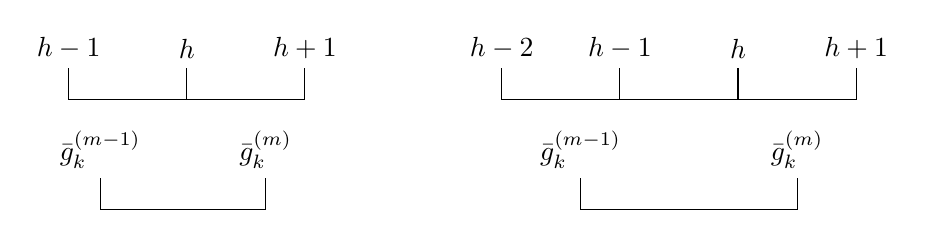
\begin{tikzpicture}
		\draw (0, 2.4) node[above]{$h - 1$} -- (0, 2) -- (1.5, 2) -- (3, 2);
		\draw (5.5, 2) -- (10, 2) -- (10, 2.4) node[above]{$h + 1$};
		\draw(1.5, 2) -- (1.5, 2.4) node[above]{$h$};
		\draw(3, 2) -- (3, 2.4) node[above]{$h + 1$};
		\draw(5.5, 2) -- (5.5, 2.4) node[above]{$h - 2$};
		\draw(7, 2) -- (7, 2.4) node[above]{$h - 1$};
		\draw(8.5, 2) -- (8.5, 2.4) node[above]{$h$};
		\draw (0.4, 1) node[above]{$\bar{g}_k^{(m - 1)}$} -- (0.4, 0.6) -- (2.5, 0.6) -- (2.5, 1) node[above]{$\bar{g}_k^{(m)}$};
		\draw (6.5, 1) node[above]{$\bar{g}_k^{(m - 1)}$} -- (6.5, 0.6) -- (9.25, 0.6) -- (9.25, 1) node[above]{$\bar{g}_k^{(m)}$};
	\end{tikzpicture}
\caption{Two ways in which a normalised particle weight taking values between $[1/N, 2/N]$ can overlap stratification intervals.}
\label{fig:max_weight}
\end{figure}
\noindent
For a given length $g_k^{(m)} - g_k^{(m - 1)}$, the product of overlaps in the left panel of Figure \ref{fig:max_weight} is minimised by aligning $g_k^{(m)}$ with $(h + 1) / N$, or equivalently $g_k^{(m - 1)}$ with $(h - 1) / N$, yielding
\begin{align}
\Big| \Big[ \frac{ h - 1 }{ N }, \frac{ h }{ N } \Big) \cap \Big[ \bar{ g }_k^{ ( m - 1 ) }, \bar{ g }_k^{ ( m ) } \Big) \Big| &\Big| \Big[ \frac{ h }{ N }, \frac{ h + 1 }{ N } \Big) \cap \Big[ \bar{ g }_k^{ ( m - 1 ) }, \bar{ g }_k^{ ( m ) } \Big) \Big| \notag \\
&\geq \Big(g_k^{(m)} - g_k^{(m - 1)} - \frac{1}{N}\Big) \frac{1}{N} \geq \frac{\varepsilon_N}{N}. \label{max_weight_bound_1}
\end{align}
The right panel yields the same bound after summing up the two successive pairs $(h - 2, h - 1)$ and $(h - 1, h)$:
\begin{align}
&\Big| \Big[ \frac{ h - 2 }{ N }, \frac{ h - 1 }{ N } \Big) \cap \Big[ \bar{ g }_k^{ ( m - 1 ) }, \bar{ g }_k^{ ( m ) } \Big) \Big| \Big| \Big[ \frac{ h - 1 }{ N }, \frac{ h }{ N } \Big) \cap \Big[ \bar{ g }_k^{ ( m - 1 ) }, \bar{ g }_k^{ ( m ) } \Big) \Big| \notag \\
&\phantom{\geq}+ \Big| \Big[ \frac{ h - 1 }{ N }, \frac{ h }{ N } \Big) \cap \Big[ \bar{ g }_k^{ ( m - 1 ) }, \bar{ g }_k^{ ( m ) } \Big) \Big| \Big| \Big[ \frac{ h }{ N }, \frac{ h + 1 }{ N } \Big) \cap \Big[ \bar{ g }_k^{ ( m - 1 ) }, \bar{ g }_k^{ ( m ) } \Big) \Big| \notag \\
&= \Big(g_k^{(m)} - g_k^{(m - 1)} - \frac{1}{N}\Big) \frac{1}{N} \geq \frac{\varepsilon_N}{N}. \label{max_weight_bound_2}
\end{align}
Moreover, the inequalities on the right-hand sides of \eqref{max_weight_bound_1} and \eqref{max_weight_bound_2} continue to hold if $\varepsilon_N > 1/N$, albeit with more terms to sum on the left-hand sides.
Substituting both into \eqref{stratified_lb_start} yields
\begin{align}
&\bbP^{ \bfX }( | \bar{ G }_k^{ N, n } | < | \xi | | \bar{ G }_{ k - 1 }^{ N, n } = \xi, G_j^{ N, n } = ( \xi, \ell_0 ) ) \notag \\
&\geq \sum_{ \ell_1 \in [ N ]_d^{ | \xi | } } \bbP^{ \bfX }( G_{ k - 1 }^{ N, n } = ( \xi, \ell_1 ) | \bar{ G }_{ k - 1 }^{ N, n } = \xi, G_j^{ N, n } = ( \xi, \ell_0 ) ) \frac{ N^2 }{ ( N )_2 \gamma^2 } \frac{\varepsilon_N}{N} \notag \\
&= \frac{ 1 + o( 1 ) }{ \gamma^2 } \frac{\varepsilon_N}{N}, \label{stratified_lb}
\end{align}
which is bounded away from zero in $k$ for each fixed $N$.
Hence, for a fixed $t \in (0, \infty)$, we have $\bbP( \tau_N( \xi, \ell, j; t ) = \infty ) \to 0$ as $N \to \infty$ as required.

Finally, the bounds on the timescale $\tau_N(t)$ in \eqref{stratified_timescale_lb} and \eqref{stratified_timescale_ub} follow from \eqref{eq:stratified_merger_ub} and \eqref{stratified_lb}, as well as \eqref{binomial_sum}.
\end{proof}

\end{document}
